%%%%%%
%BASE
%%%
\documentclass[12pt,a4paper]{article}
\usepackage[utf8]{inputenc}
\usepackage[T1]{fontenc}
\usepackage[francais]{babel}
\frenchbsetup{StandardLists=true} % à inclure si on utilise \usepackage[french]{babel}
\usepackage{enumitem}
\usepackage{graphicx}

%%%%%
%MATHS
%%%
\usepackage{amsmath}
\usepackage{array}
\usepackage{ntheorem}

%%%%%
%COULEURS
%%%
\usepackage{xcolor}
\usepackage{color}
\usepackage{colortbl}

%%%%%
%PUCES
%%%
\usepackage{pifont}

\everymath{\displaystyle}
\usepackage{hyperref}
\setlength{\parindent}{10px}

%%%%%
%Tableau
%%%
\usepackage{multirow}
% Permet d'agrandir le tableau.
\renewcommand{\arraystretch}{1.5}
\setlength{\tabcolsep}{1cm}




%%%%%
%Haut de Page
%%%
\usepackage{fancybox}
\usepackage{fancyhdr}
\usepackage[left=1.3cm,right=1.2cm,top=2cm,bottom=1.5cm]{geometry}
\pagestyle{fancy}
\fancyhead[L]{Lespinasse Florentin}
\fancyhead[C]{Géographie}
\fancyhead[R]{1STI2D4~~~~~~~~\today}


\begin{document}
\begin{center}
        \shadowbox{\begin{large}
                \textcolor{red}{G3 Des espaces rureaux aux fonctions de plus en plus variées}
        \end{large}}
    \end{center}
    \vspace{0.5 cm}

\centering
\textcolor{red}{Introduction}\par
\flushleft
Espace rural est défini par rapport à ce qui n’est pas urbain : une présence importante de formations végétales telles que les forêts, les cultures ou les prairies. 
Il est aussi caractérisé par sa fonction agricole et sa faible densité.\par

Ces espaces connaissent d’importantes transformations : la place de l’agriculture reste importante mais ils sont de plus en plus liés aux espaces urbains.
Leurs fonctions se diversifient : fonctions résidentielles, industrielles, environnementales, touristiques.\\ 
    \vspace{0.5 cm}

\textbf{\textcolor{green}{Definition $\rightarrow$ }
Espace rural} : Espace dans lequel l’occupation du sol par la végétation et l’activité agricole sont importantes. C’est généralement un espace de faible densité.\par
    \vspace{0.5 cm}
\centering
\textcolor{blue}{\textbf{ Problématique}: Quels sont les fonctions aujourd'hui des espaces rureaux?}
\flushleft

\begin{enumerate}[label=\Roman*.,font=\color{red}]
\item	\textcolor{red}{\textbf{Une activité agricole encore très importante dans les espaces rureaux}}
\begin{center}
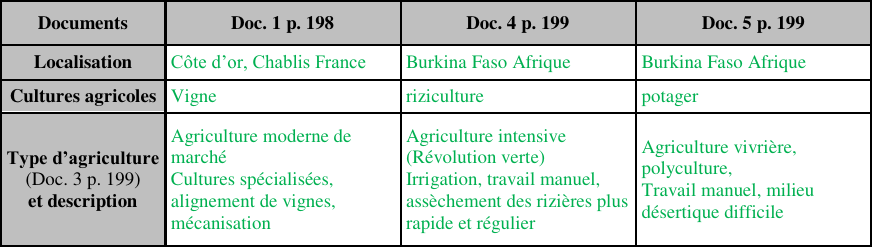
\includegraphics[scale=0.5]{I_G3.png}
\end{center}

\textbf{\textcolor{green}{Definition $\rightarrow$ }
Agriculture intensive} : Agriculture à forte production par unité de surface.\par
\textbf{Agriculture extensive} : agriculture basée sur l’exploitation de surfaces très importantes.\par


\item \textcolor{red}{\textbf{Des espaces rureaux marqués par une diversité des fonctions }}
\begin{center}
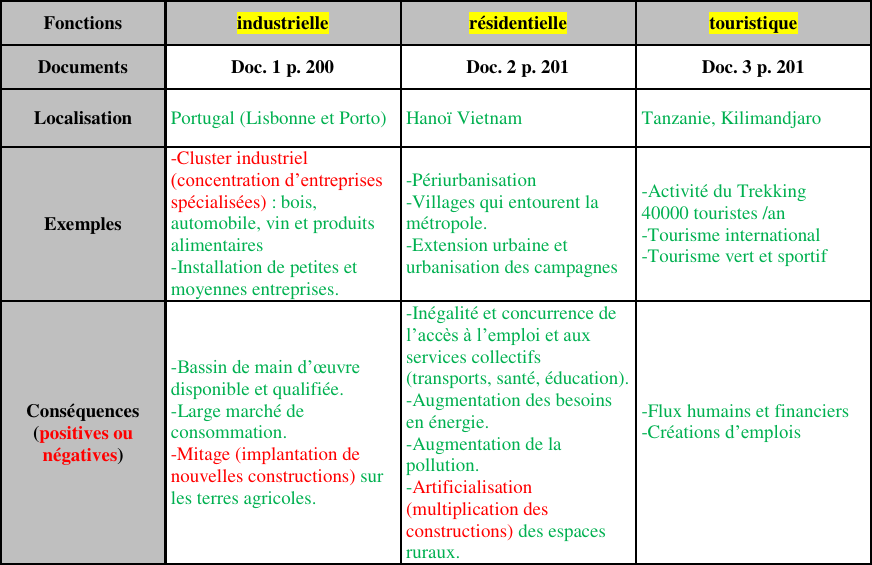
\includegraphics[scale=0.5]{II_G3.png}
\end{center}
\item \textcolor{red}{\textbf{															}}



\end{enumerate}

\end{document}

